\documentclass[conference]{IEEEtran}
\IEEEoverridecommandlockouts
% The preceding line is only needed to identify funding in the first footnote. If that is unneeded, please comment it out.
\usepackage{cite}
\usepackage{amsmath,amssymb,amsfonts}
\usepackage{float}
\usepackage[a4paper, top=19mm, bottom=43mm, left=14.3mm, right=14.3mm]{geometry} 
\usepackage{algorithmic}
\usepackage{graphicx}
\usepackage{textcomp}
\usepackage{xcolor}
\usepackage{tabularray}
\def\BibTeX{{\rm B\kern-.05em{\sc i\kern-.025em b}\kern-.08em
    T\kern-.1667em\lower.7ex\hbox{E}\kern-.125emX}}
\begin{document}

\title{Automatic Question Generation from Handwritten Lecture Notes on
KeyBERT-indexed T5-TrOCR Pipeline Using BERTscore Evaluation}
\author{\IEEEauthorblockN{Rommel John Ronduen\textsuperscript{1}, Jan Adrian Manzanero\textsuperscript{2}, Analyn Yumang\textsuperscript{3}}
\IEEEauthorblockA{\textit{School of Electrical, Electronics, and Computer Engineering} \\
\textit{Mapua University}\\
Manila, Philippines 1002\\
\textsuperscript{1}\texttt{rjhronduen@mymail.mapua.edu.ph}\\ 
\textsuperscript{2}\texttt{jacmanzanero@mymail.mapua.edu.ph}\\ 
\textsuperscript{3}\texttt{anyumang@mapua.edu.ph}}
}

\maketitle

\begin{abstract}
This research improves on an automatic question generation (AQG) system 
that utilizes optical character recognition (OCR) from handwritten 
lecture notes as a context source for generating questions. Such system 
utilizes the Text-to-Text transformer (T5) for AQG and Transformer-based 
Optical Character Recognition (TrOCR) for the OCR with the use of 
the Gemini 1.5 Flash large language model (LLM) for text 
correction and enhancement. A version of the Bidirectional Encoder 
Representations from Transformers (BERT) called KeyBERT was used for 
the extraction of relevant phrases and keywords from the extracted 
information as bases for question generation. The system utilizes 
a Raspberry Pi 5 equipped with a Logitech C922 web camera and
touchscreen liquid crystal display (LCD). A web application was 
developed using Angular and Flask for prototyping in allowing for 
the AQG process for experimentation. The system achieved an 
85.1\% question validity while achieving an average 64.1\% precision, 
59.77\% recall, and 61.67\% F1 score using BERTscore semantic 
analysis versus student-made questions on undergraduate level computer networks and 
cybersecurity. This system produces questions of decent context capture 
but with recommended improvements on hardware, model parameter size, and 
image preprocessing techniques.
\end{abstract}
\begin{IEEEkeywords}
Automatic Question Generation, Optical Character Recognition,
BERT, T5, Raspberry Pi
\end{IEEEkeywords}
%BEGIN INTRODUCTION
\section{Introduction}
Handwritten lecture notes are still widely used in educational institutions.
Since the advent of artificial intelligence (AI), education has become
the primary focus of AI research. AI has been used to automate several processes,
and one which is the generation of learning materials such as questions in the
form of quizzes. Literature defines automatic question generation (AQG) as the
process of generating questions from a given text. \\
\indent No AQG implementation involved the process of optical character
recognition (OCR) for the extraction of text content from handwritten lecture 
notes with semantic evaluation. For instance, \cite{Gaur2023} provided 
AQG from programming source code where a user interface allows for user 
text input and shows the generated questions. In a correlational study of AQG 
to student learning \cite{Tsai2021}, an AQG implementation used existing text files with 
the Bidirectional Encoder Representations from Transformers (BERT) 
for keyword extraction, and the T5 model for the generation of questions.
Another AQG implementation utilized video media \cite{Ou2022} where audio recognition led 
to transcript generation that was used for AQG through the Bidirectional 
and Auto-Regressive Transformer (BART). In addressing the lack of OCR 
in existing AQG implementations, there are types of models that can be 
used which are founded by convolutional neural networks 
(CNNs). CNNs can be used for general classification \cite{Manlises2024}
\cite{Calimag2023}. For instance, 
MobileNetv2 and VGG-16 are types of CNNs that can classify 
medicinal mushrooms \cite{Sutayco2023}. These CNNs consist of 
different layers that perform transformations from the input image 
that leads to extraction of features used for inferencing \cite{Estrella2024}
\cite{Wata2023}. In evaluating CNNs, confusion matrices provide an illustration and computation 
of accuracy \cite{Bacalla2023} \cite{Baguisi2024}. OCR can be made possible
through CNNs by means of proper image capture. For instance, Baybayin 
characters were properly recognized \cite{Ligsay2022}. However, 
OCR technology has advanced to the point where transformers are now used 
through the Transformer-based Optical Character Recognition (TrOCR) model. 
This is a model utilizes an encoder-decoder framework in parsing through 
images of text lines and producing corresponding strings \cite{Li2021}. 
Due to its pre-trained availability and seamless implementation to 
Python, this model was chosen in this research. In performing question
generation, the researchers realized BERT and T5. With BERT, 
the model comes pre-trained that can be utilized in text classification
and indexing \cite{Fernandez2023} \cite{Mingua2021}. 
BERT comes pre-trained, meaning it is 
immediately capable of extracting semantic features from 
text for inferencing \cite{Liu2023}. Due to the fine-tuning 
offered by BERT, many versions of BERT have been realized 
that serve different specialized purposes \cite{Patra2024}. 
KeyBERT is a variant of BERT that was fine-tuned for extracting 
relevant words and phrases in a paragraph through cosine 
similarity of inferred candidate structures in the text. 
KeyBERT has been used in an implementation of AQG \cite{Talupuri2024}
in producing multiple-choice questions where the choices are 
indexed by KeyBERT. Apart from generative purposes, BERT can be 
used for evaluation through BERTscore semantic analysis. 
Since BERT can be used to understand the meaning between a reference 
and generated text result, BERTscore can infer the similarity 
among sentences and provide recall and precision metrics based on
the meaning of the sentences \cite{Zhang2019} which $n$-gram overlap 
methods cannot realize. In total, this research addresses 
the lack of OCR in AQG implementations by means of TrOCR and 
Gemini 1.5 Flash for text enhancement for 
text extraction from handwritten lecture notes while utilizing 
T5 and KeyBERT for AQG with semantic evaluation through 
BERTscore.\\
\indent The general objective of this research is to allow AQG from 
handwritten lecture notes on a KeyBERT-indexed T5-TrOCR algorithm pipeline 
evaluated through BERTscore semantic analysis. More specifically, 
this research aims to utilize KeyBERT indexing for extracting 
relevant keywords and phrases coming from the extracted text 
through TrOCR and Gemini 1.5 Flash as basis for AQG through the base model T5 fine-tuned 
on the Stanford Question Answering Dataset (SQuADv1.1). 
Moreover, this research aims to utilize a Raspberry Pi 5 on the 8 gigabyte 
memory version alongside a Logitech C922 web camera and Waveshare touchscreen 
LCD in facilitating the necessary inputs and outputs for the system through
a constructed enclosure with proper lighting. Lastly, this research 
aims to evaluate the quality of AQG by means of KeyBERT semantic analysis 
and the question validity rate through manual analysis. \\ 
\indent This research is limited by the consideration of only 
single-column, diagram and equation free, and English handwritten lecture notes 
of no erasures on strictly letter-sized plain sheet paper.
Moreover, the system is confined to the 
use of the T5-TrOCR pipeline utilizing the base versions while 
also utilizing the SQuADv1.1 dataset for the fine-tuning. It is also important 
to note that the system is limited to the facilitation of the processes in 
the hardware of the 8-gigabyte version of the Raspberry Pi 5. The use of 
a higher parameter count for the T5 and TrOCR models and the use of a different 
dataset for fine-tuning may allow for differing results. Lastly, the 
utilization of a different hardware setup may also lead to alternative, if not, 
better results in terms of processing time. 
%BEGIN II
\section{Materials and Methods}
    \subsection{Hardware Development}
        \subsubsection{System Block Diagram}
            \hfill \\
            \vspace{-0.6cm}
            \begin{figure}[H]
                \centerline{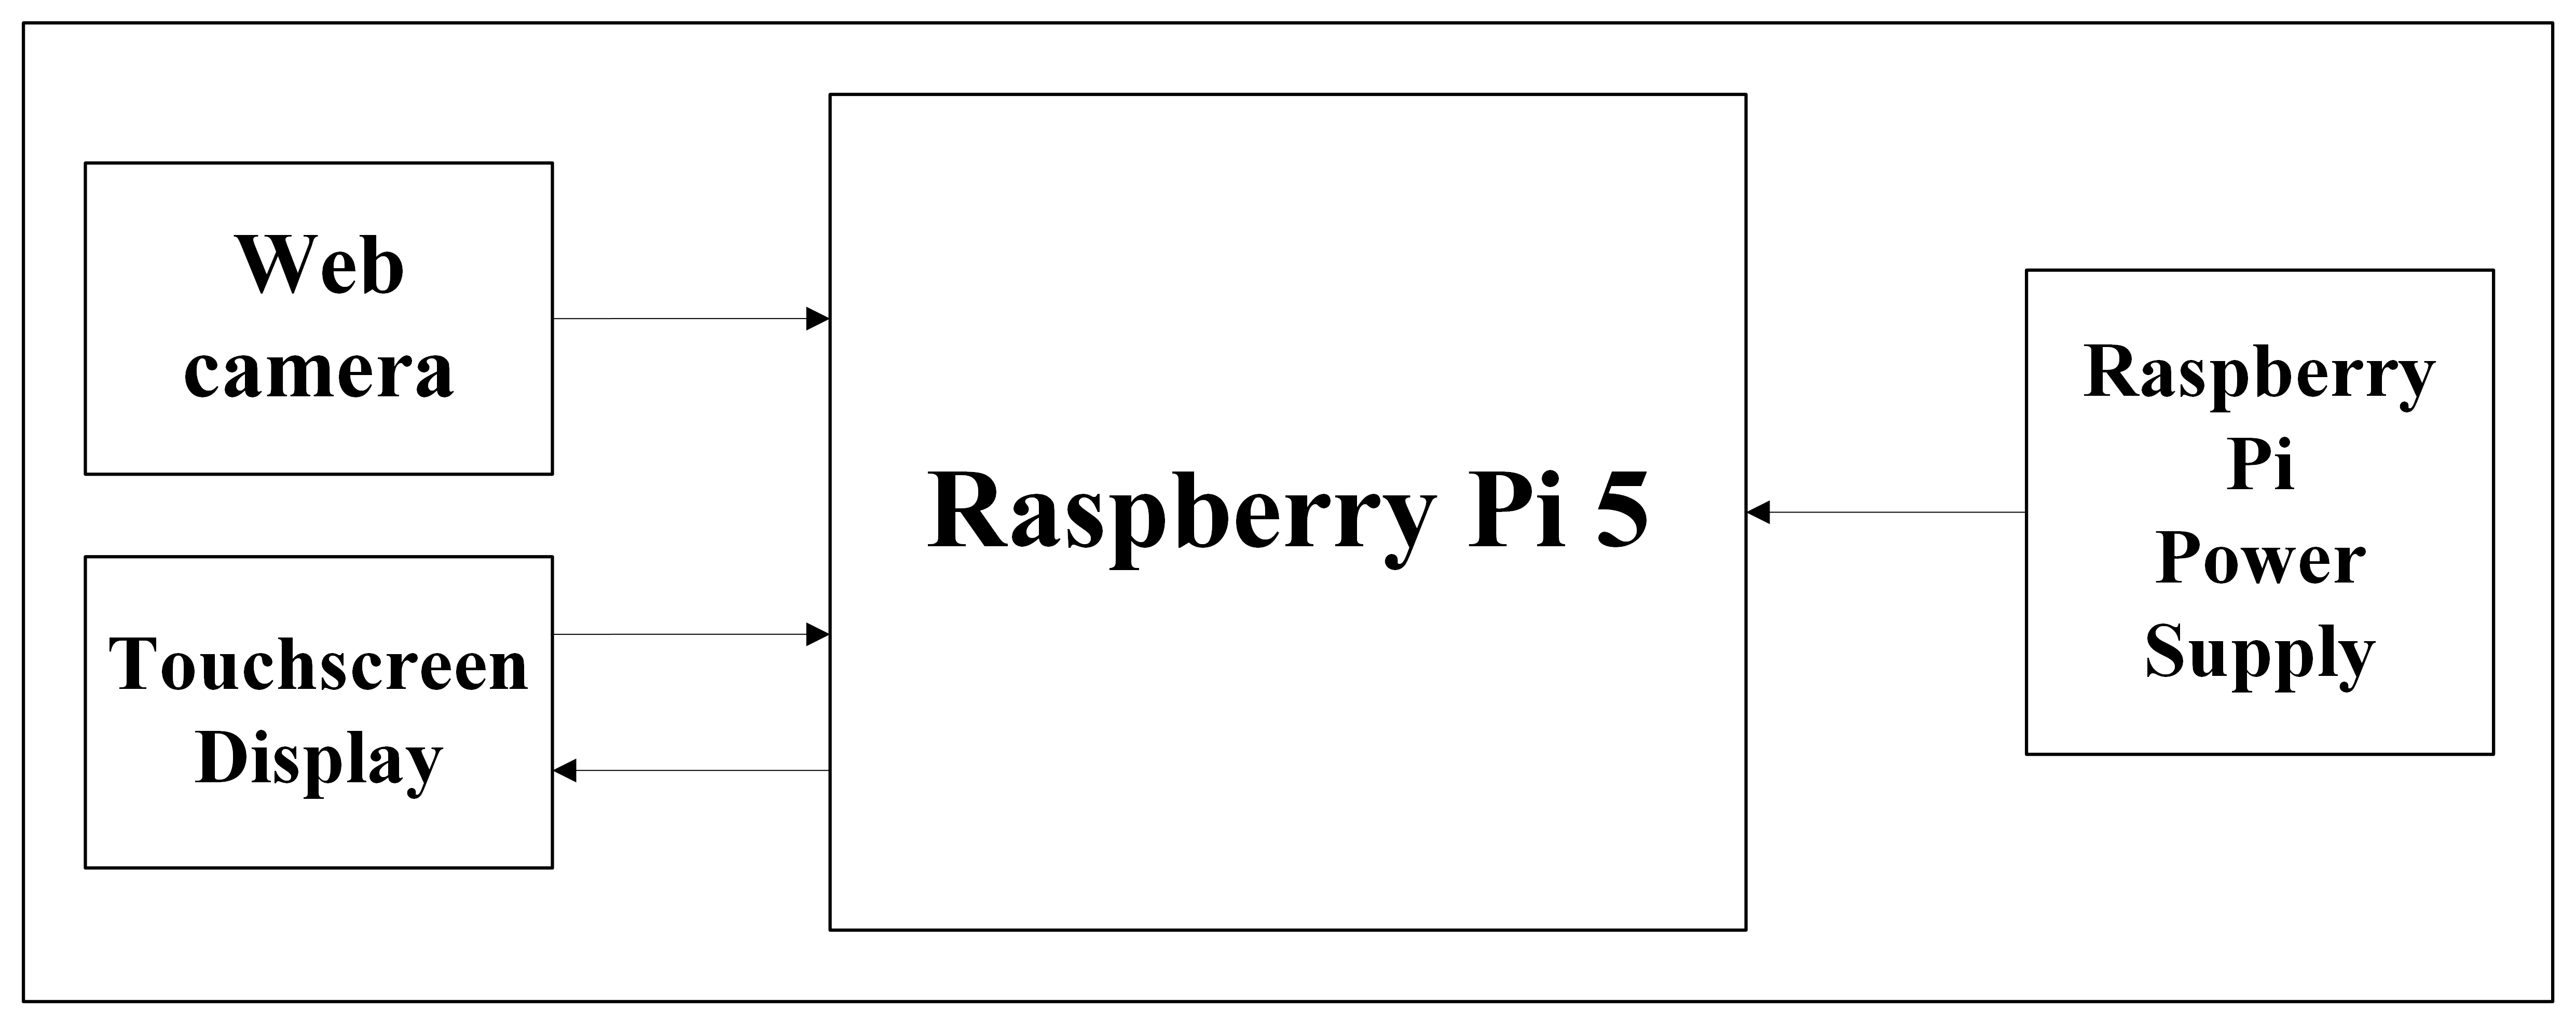
\includegraphics[width=3.0in]{blockdiag.png}}
                \vspace{-0.3cm}
                \caption{System block diagram.} 
                \label{blockdiagram}
            \end{figure} 
            \vspace{-0.4cm}
            \newpage
            \indent The system block diagram is shown in Fig. 
            \ref{blockdiagram}. The system is composed of a 
            Raspberry Pi 5, a web camera, and a 
            touchscreen monitor. The Raspberry Pi 5 is the main 
            processing unit of the system. The web camera is 
            used for capturing images of handwritten lecture notes. 
            The touchscreen monitor is used for displaying the 
            generated questions. The system is enclosed in a box 
            with proper illumination for the facilitation of the 
            processes.
        \vspace{0.2cm}
        \subsubsection{Experimental Setup}
            \hfill \\
            \vspace{-0.6cm}
            \begin{figure}[H]
                \centerline{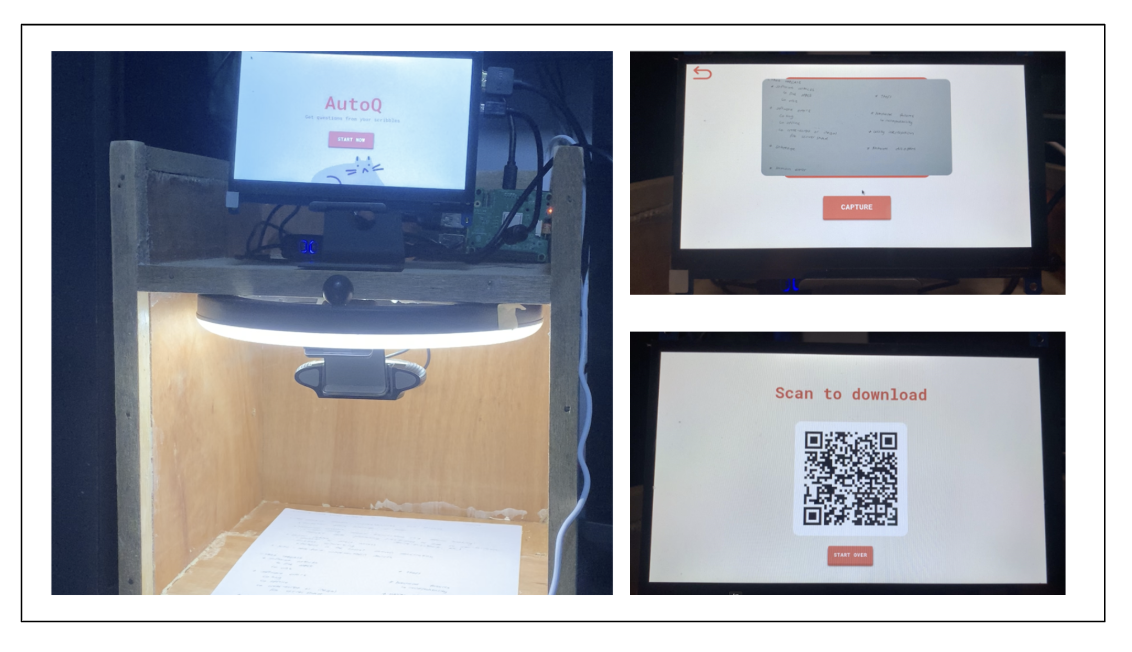
\includegraphics[width=3.6in]{experimental.png}}
                \vspace{-0.3cm}
                \caption{Experimental setup.} 
                \label{experimental}
            \end{figure} 
            \vspace{-0.3cm}
            \indent The experimental setup is shown in 
            Fig. \ref{experimental}. The system is enclosed in a
            constructed wooden box with proper illumination. The
            Raspberry Pi 5 is connected to the web camera and the
            touchscreen monitor. The web camera is used for capturing
            images of handwritten lecture notes. The touchscreen
            monitor is used for guiding the user in the system
            processes.
    \subsection{Software Development}
        \subsubsection{System Flowchart}
            \hfill 
            \begin{figure}[H]
                \centerline{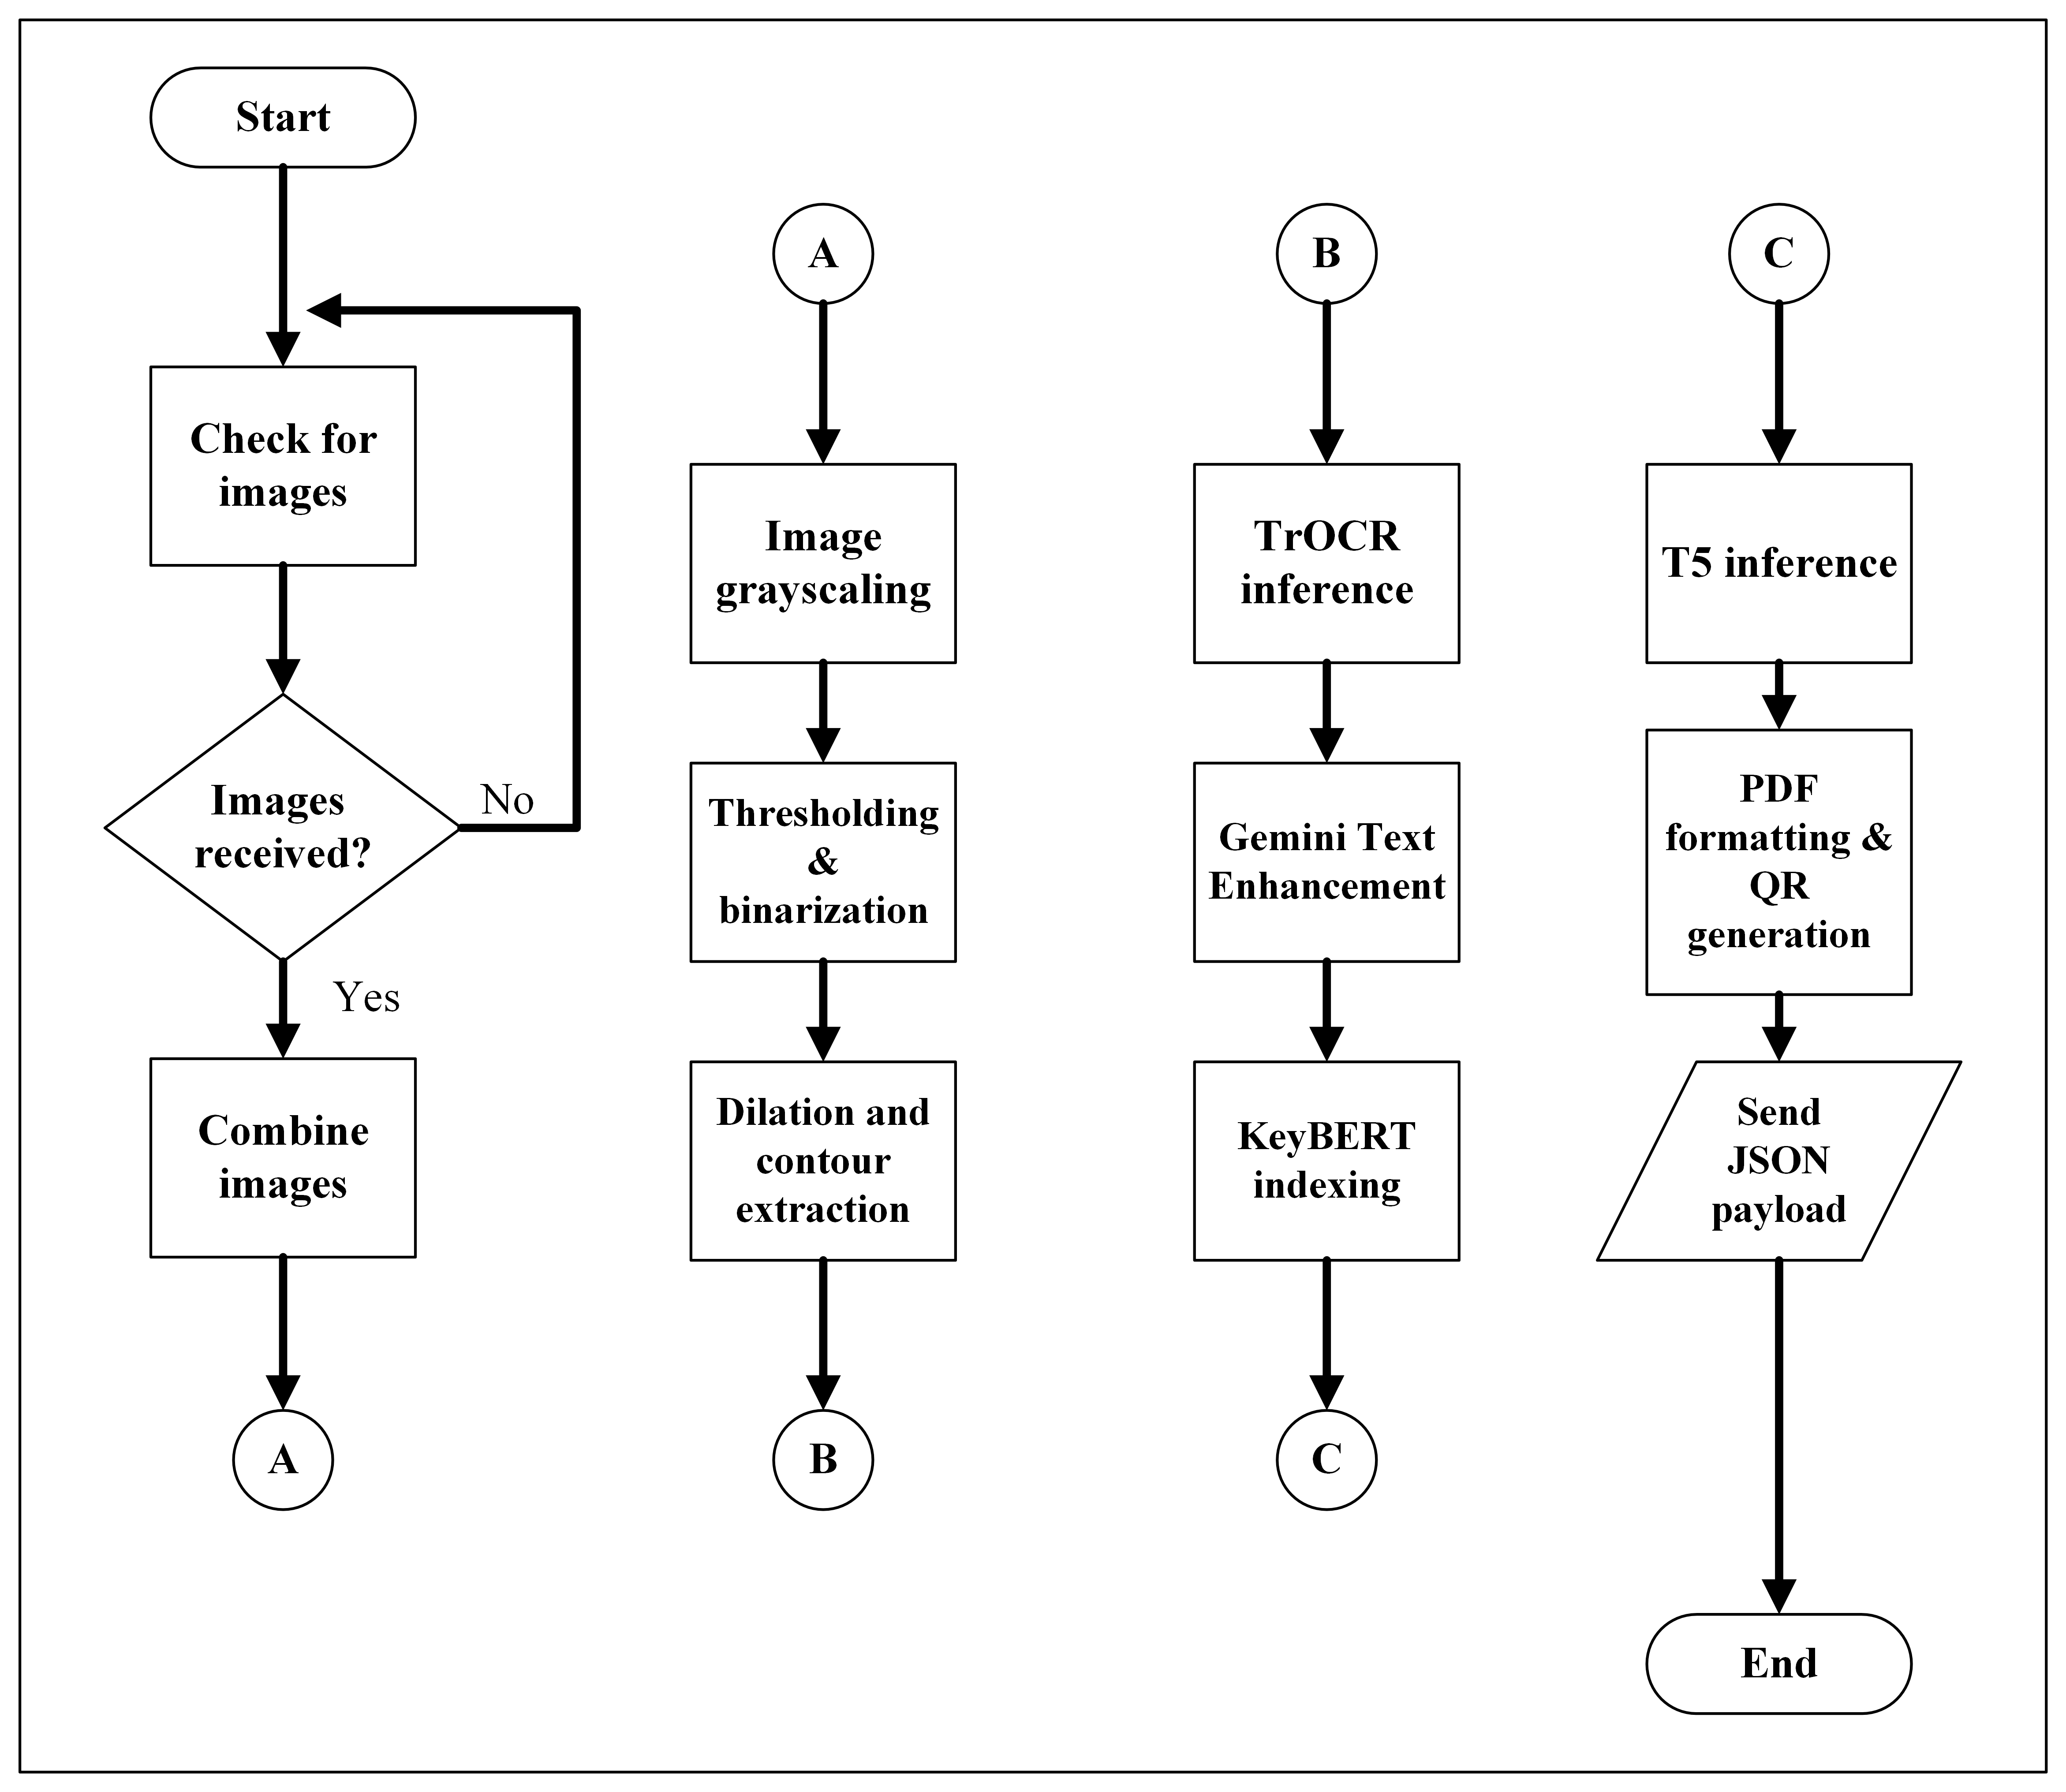
\includegraphics[width=3.6in]{flowchart.png}}
                \vspace{-0.4cm}
                \caption{System flowchart.} 
                \label{flowchart}
            \end{figure}
            \indent The system flowchart is shown in 
           Fig. \ref{flowchart}. The system 
           starts by collecting
           the image captures of the top and bottom halves 
           of the notes. The image captures are then
           combined and undergone a series of image 
           transformations that extracted the text lines. 
           These text lines were inputted to the TrOCR for 
           inferencing and the extracted text is then
           inputted to the T5 for AQG. The generated
           questions are formatted to a portable document
              format (PDF) and uploaded to Google Drive 
            where a quick response (QR) code is generated for the user to download 
            the PDF on their device. A JavaScript 
            Object Notation (JSON) payload is then sent 
            to the front end of the system for the 
            notification on the touchscreen display.
        \vspace{0.4cm}
        \subsubsection{T5 AQG}
        \hfill \\
            \indent In this research, T5 was fine-tuned 
            to the SQuADv1.1 dataset. The input features 
            considered were the context and the chosen 
            answer phrase/keyword. The output feature
            was the question generated from the context
            and the chosen answer phrase/keyword. 
            
    \subsection{Data Gathering}
        \hfill \\
        \vspace{-1cm}
        \begin{figure}[H]
            \centerline{\includegraphics[width=3in]{datacollection.png}}
            \vspace{-0.3cm}
            \caption{Sample captured notes (with processed version on right).} 
            \label{datacollection}
        \end{figure} 
        \vspace{-0.3cm} 
        \indent A sample capture from the procured testing dataset 
        is shown in Fig. \ref{datacollection}. 
        A total of 70 handwritten lecture notes were collected
        from an undergraduate class on computer networking and 
        cybersecurity. These notes were inputted to the system 
        which will result in the generation of 350 questions 
        for validity testing. \\ 
        \indent Apart from the notes, the researchers collected 
        questions from students based on a summary discussion that 
        contains the top five most common keywords 
        (MAC, address, ethernet, data, frame) in the notes 
        of the students. In a class of 27 students, each 
        were asked to formulate questions that answer the five 
        common keywords. A total of 135 questions were collected 
        from the students.
    \subsection{Testing and Evaluation}
    \begin{table}[H]
        \caption{Testing and Evaluation Table for Question Validity.}
            \centering
            \begin{tblr}{
                colspec={@{}X[1] X[1] X[1] X[1]@{}}, % Makes columns flexible
                column{1} = {c}, % Align first column to center
                hlines,          % Adds horizontal lines
            }
            & \textbf{Student} & \textbf{Model} & \textbf{Validity}\\
            1 &  &  &  & \\
            ... & ... & ... & ... &\\
            350 &     &     &     & \\ 
                &   &     &  Total  &\\  % Replace X, Y, Z with actual values
            \end{tblr}
            \label{valtable}
    \end{table}
    \indent Revealed in Table \ref{valtable} is the testing 
    and evaluation of the 350 questions generated by the system 
    as a byproduct of its intake of the 70 handwritten notes 
    from the data collection. Here, an author of this research 
    in the teaching profession manually checked the questions 
    for validity. After gaining the total number of valid
    questions, it is divded by the total generated questions to 
    get the question validity rate. Mathematically: 
    \vspace{0.5cm}
    \begin{equation}
        \textrm{Validity} = \frac{\textrm{\# of valid questions}}{\textrm{\# of total questions}} \times 100\%
    \end{equation}
    \begin{table}[H]
        \caption{Testing and Evaluation Table for AQG.}
            \centering
            \begin{tblr}{
                colspec={@{}X[1] X[1] X[1] X[1] X[1] X[1] @{}}, % Makes columns flexible
                column{1} = {c}, % Align first column to center
                hlines,          % Adds horizontal lines
            }
            & \textbf{Student} & \textbf{Model} & \textbf{Recall} & \textbf{Precision} & \textbf{F1}\\
            1 &  &  &  & & & \\
            ... & ... & ... & ... & ... & ...\\
            135 &     &     &     &    & \\ 
            &   &     & Average & Average & Average\\  % Replace X, Y, Z with actual values
            \end{tblr}
            \label{aqgtable}
    \end{table}
    \indent Shown in Table \ref{aqgtable} is the testing 
    and evaluation table for AQG evaluation. For each of 
    the 135 questions from the students, the recall, 
    precision, and F1 score is calculated through 
    BERTscore.     
    \vspace{0.75cm}
    \begin{equation}
        \textrm{Recall} = \frac {1} {|x|} 
        \sum _ {\tilde{x_j}\in \tilde{x}}\max \textbf{x}_i^T \tilde{\textbf{x}}_j
    \end{equation}
    \vspace{0.75cm}
    \begin{equation}
        \textrm{Precision} = \frac {1} {|\tilde{x}|} 
        \sum _ {\tilde{x_i}\in \tilde{x}}\max \textbf{x}_i^T \tilde{\textbf{x}}_j
    \end{equation}
    \vspace{0.75cm}
    \begin{equation}
        \textrm{F1} = 2 \frac{\textrm{Precision}\cdot\textrm{Recall}}{
        \textrm{Precision} + \textrm{Recall}
        }
    \end{equation}
    \vspace{0.5cm}

    where $x$ is the reference sentence, $\tilde{x}$ is the tokenized inference sentence, 
    and $\textbf{x}_i^T\tilde{\textbf{x}}_j$ is the 
    inner product between the reference sentence vectors that 
    indicates similarity. The recall quantity
    takes the average of the best similarities across 
    the reference sentences. As for the precision, 
    it also uses the same quantities but on the 
    basis of the inference sentences $\tilde{x}$. Lastly,
    the F1 score computes the harmonic mean across (2) and (3)
    as a form of equalized score between precision and 
    recall.
\newpage
\section{Results and Discussion}
\begin{figure}[H]
    \centerline{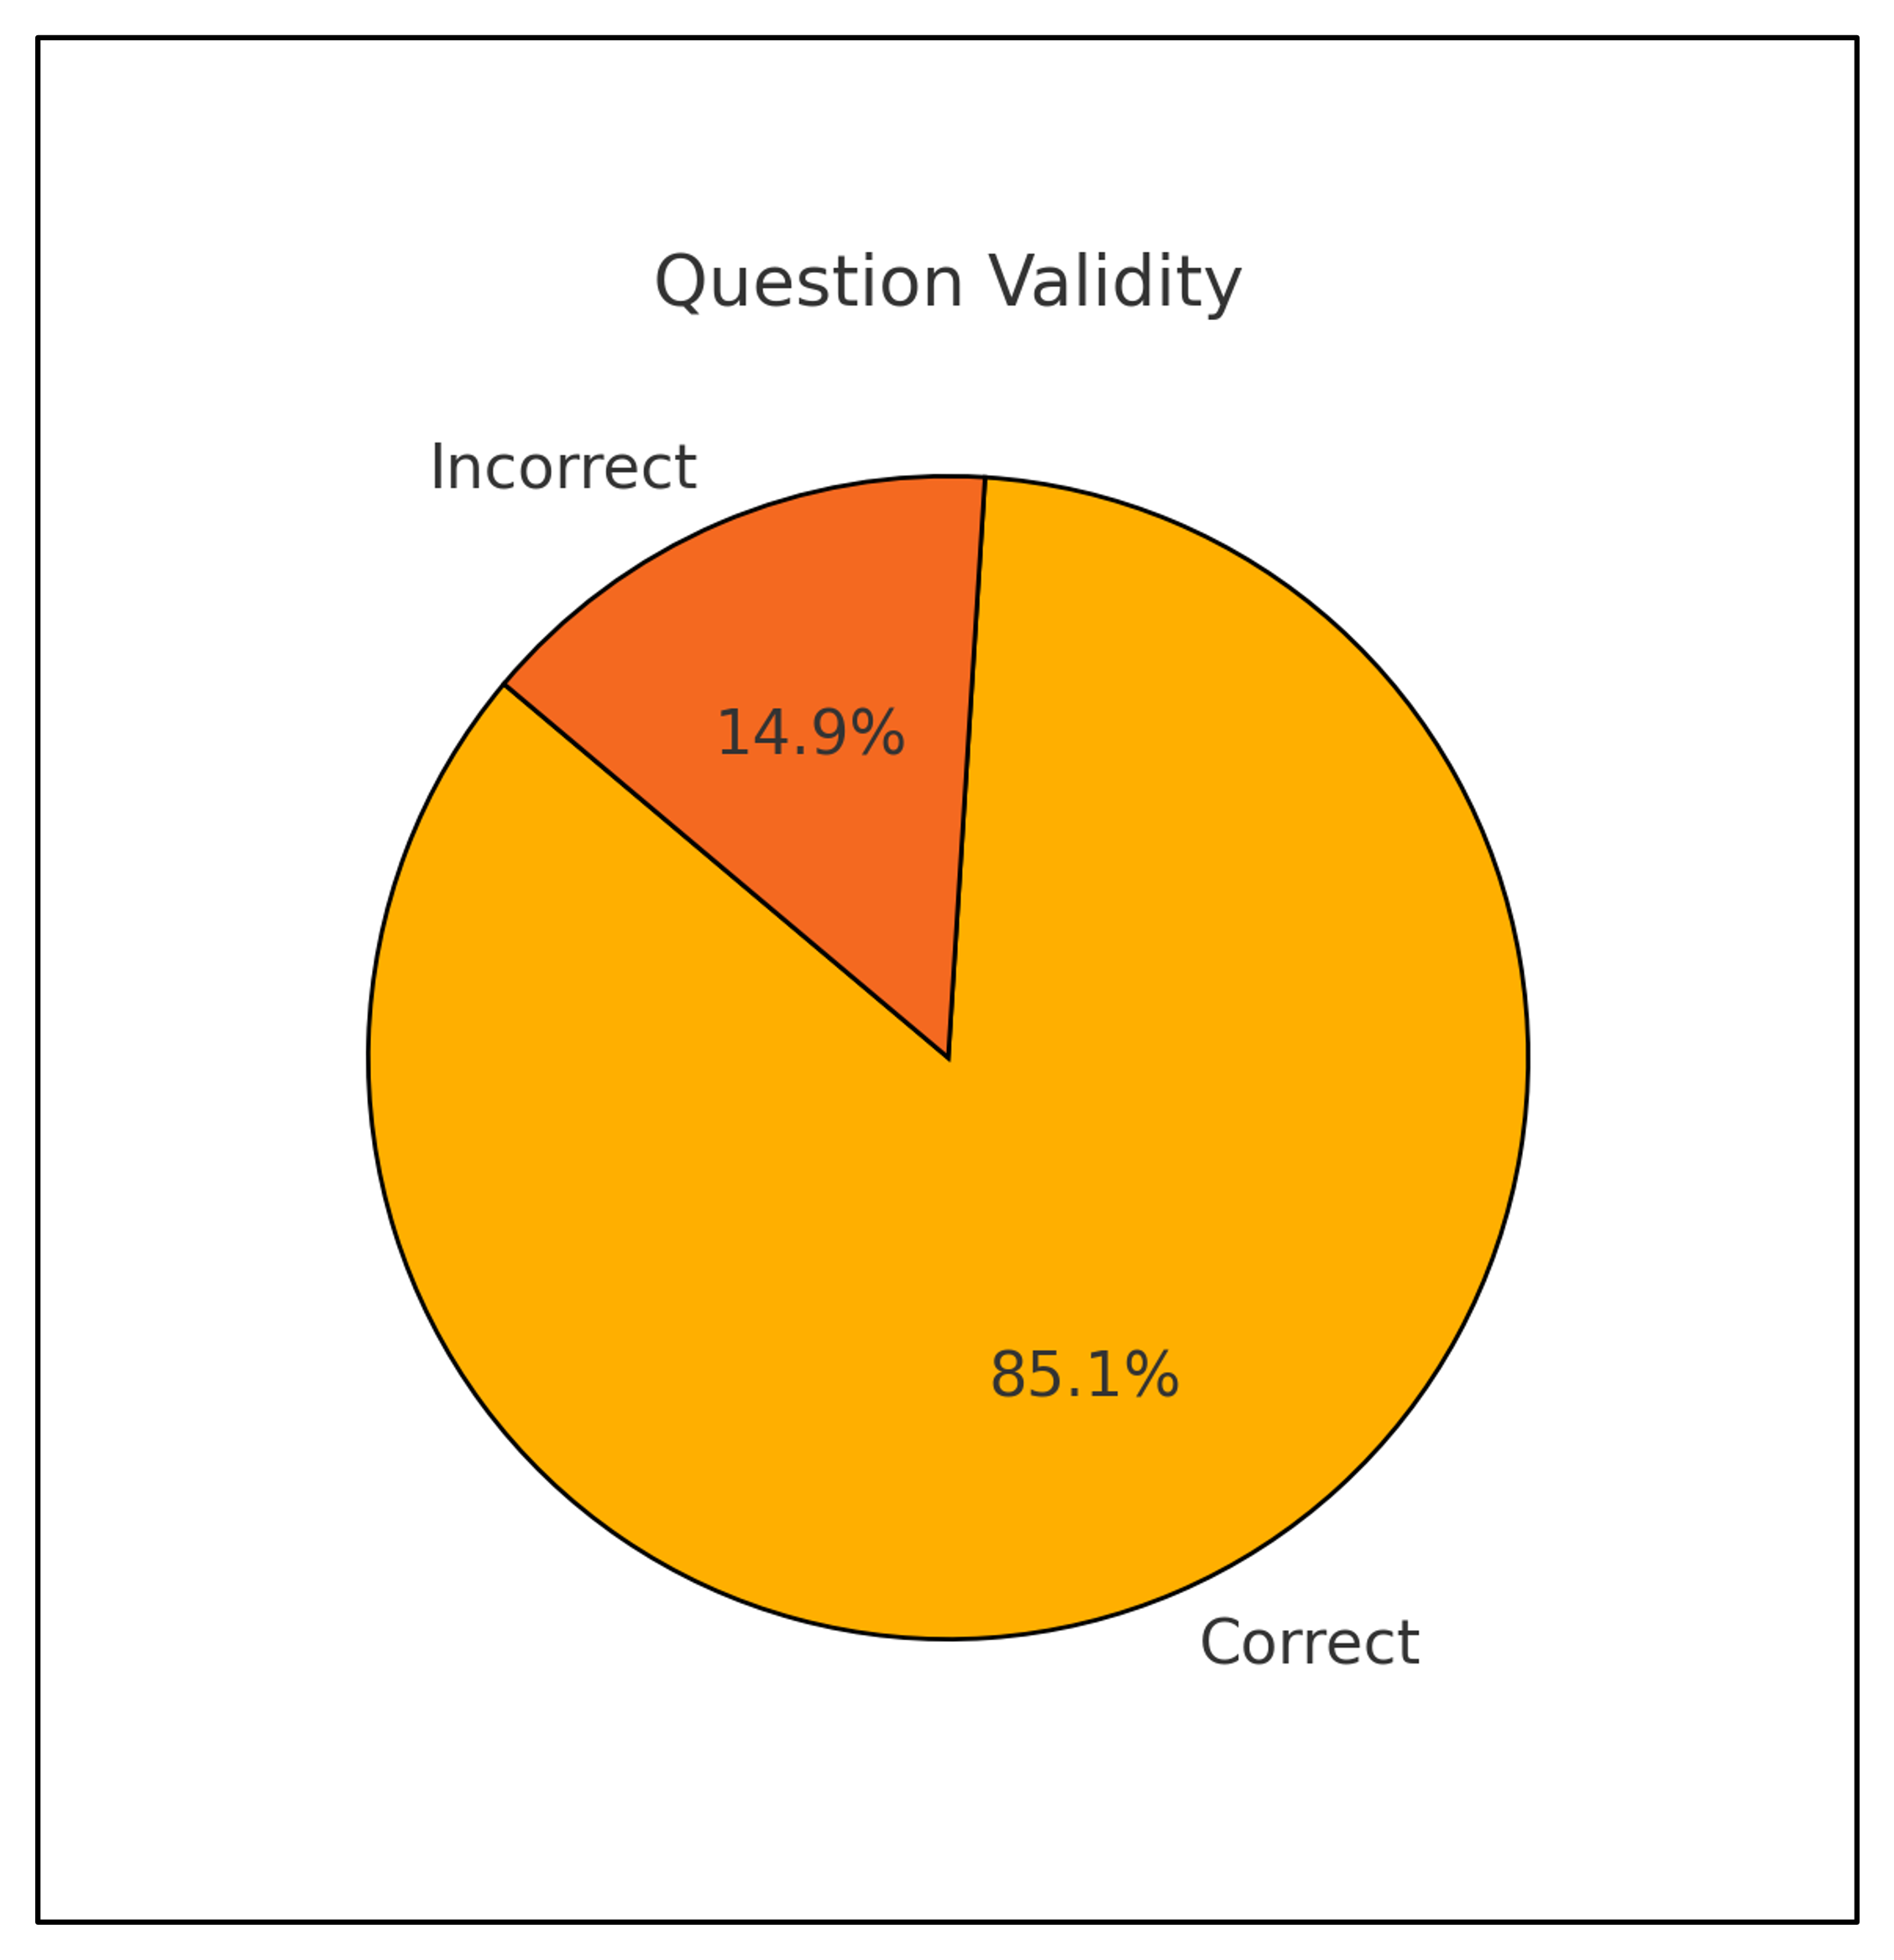
\includegraphics[width=3in]{validity.png}}
    \vspace{-0.4cm}
    \caption{Pie chart for valid questions versus invalid.} 
    \label{validity}
\end{figure}
As shown in Fig. \ref{validity}, 85.1\% of the questions generated out of 
the test set were valid in terms of logic, coherence, and 
its correlation to the answer. It means that 298 out of the 350 
questions were able to lead to the designated answer while 
providing proper structure and grammar. The use of KeyBERT 
must have allowed the T5 model to properly form the questions 
as similar to the way that SQuAD formed its questions. The 
remaining 14.9\% or 52 questions were considered invalid 
due to grammar, invalid structure, and misalignment to the 
answer it suggests. This would have been through the lack 
of parameters that T5 has in the formulation of the questions, 
since the researchers have noticed in the inferences that 
the errors in the invalid questions involve the lack of 
linking verbs, or the reveal of the answer within the question. 
\begin{figure}[H]
    \centerline{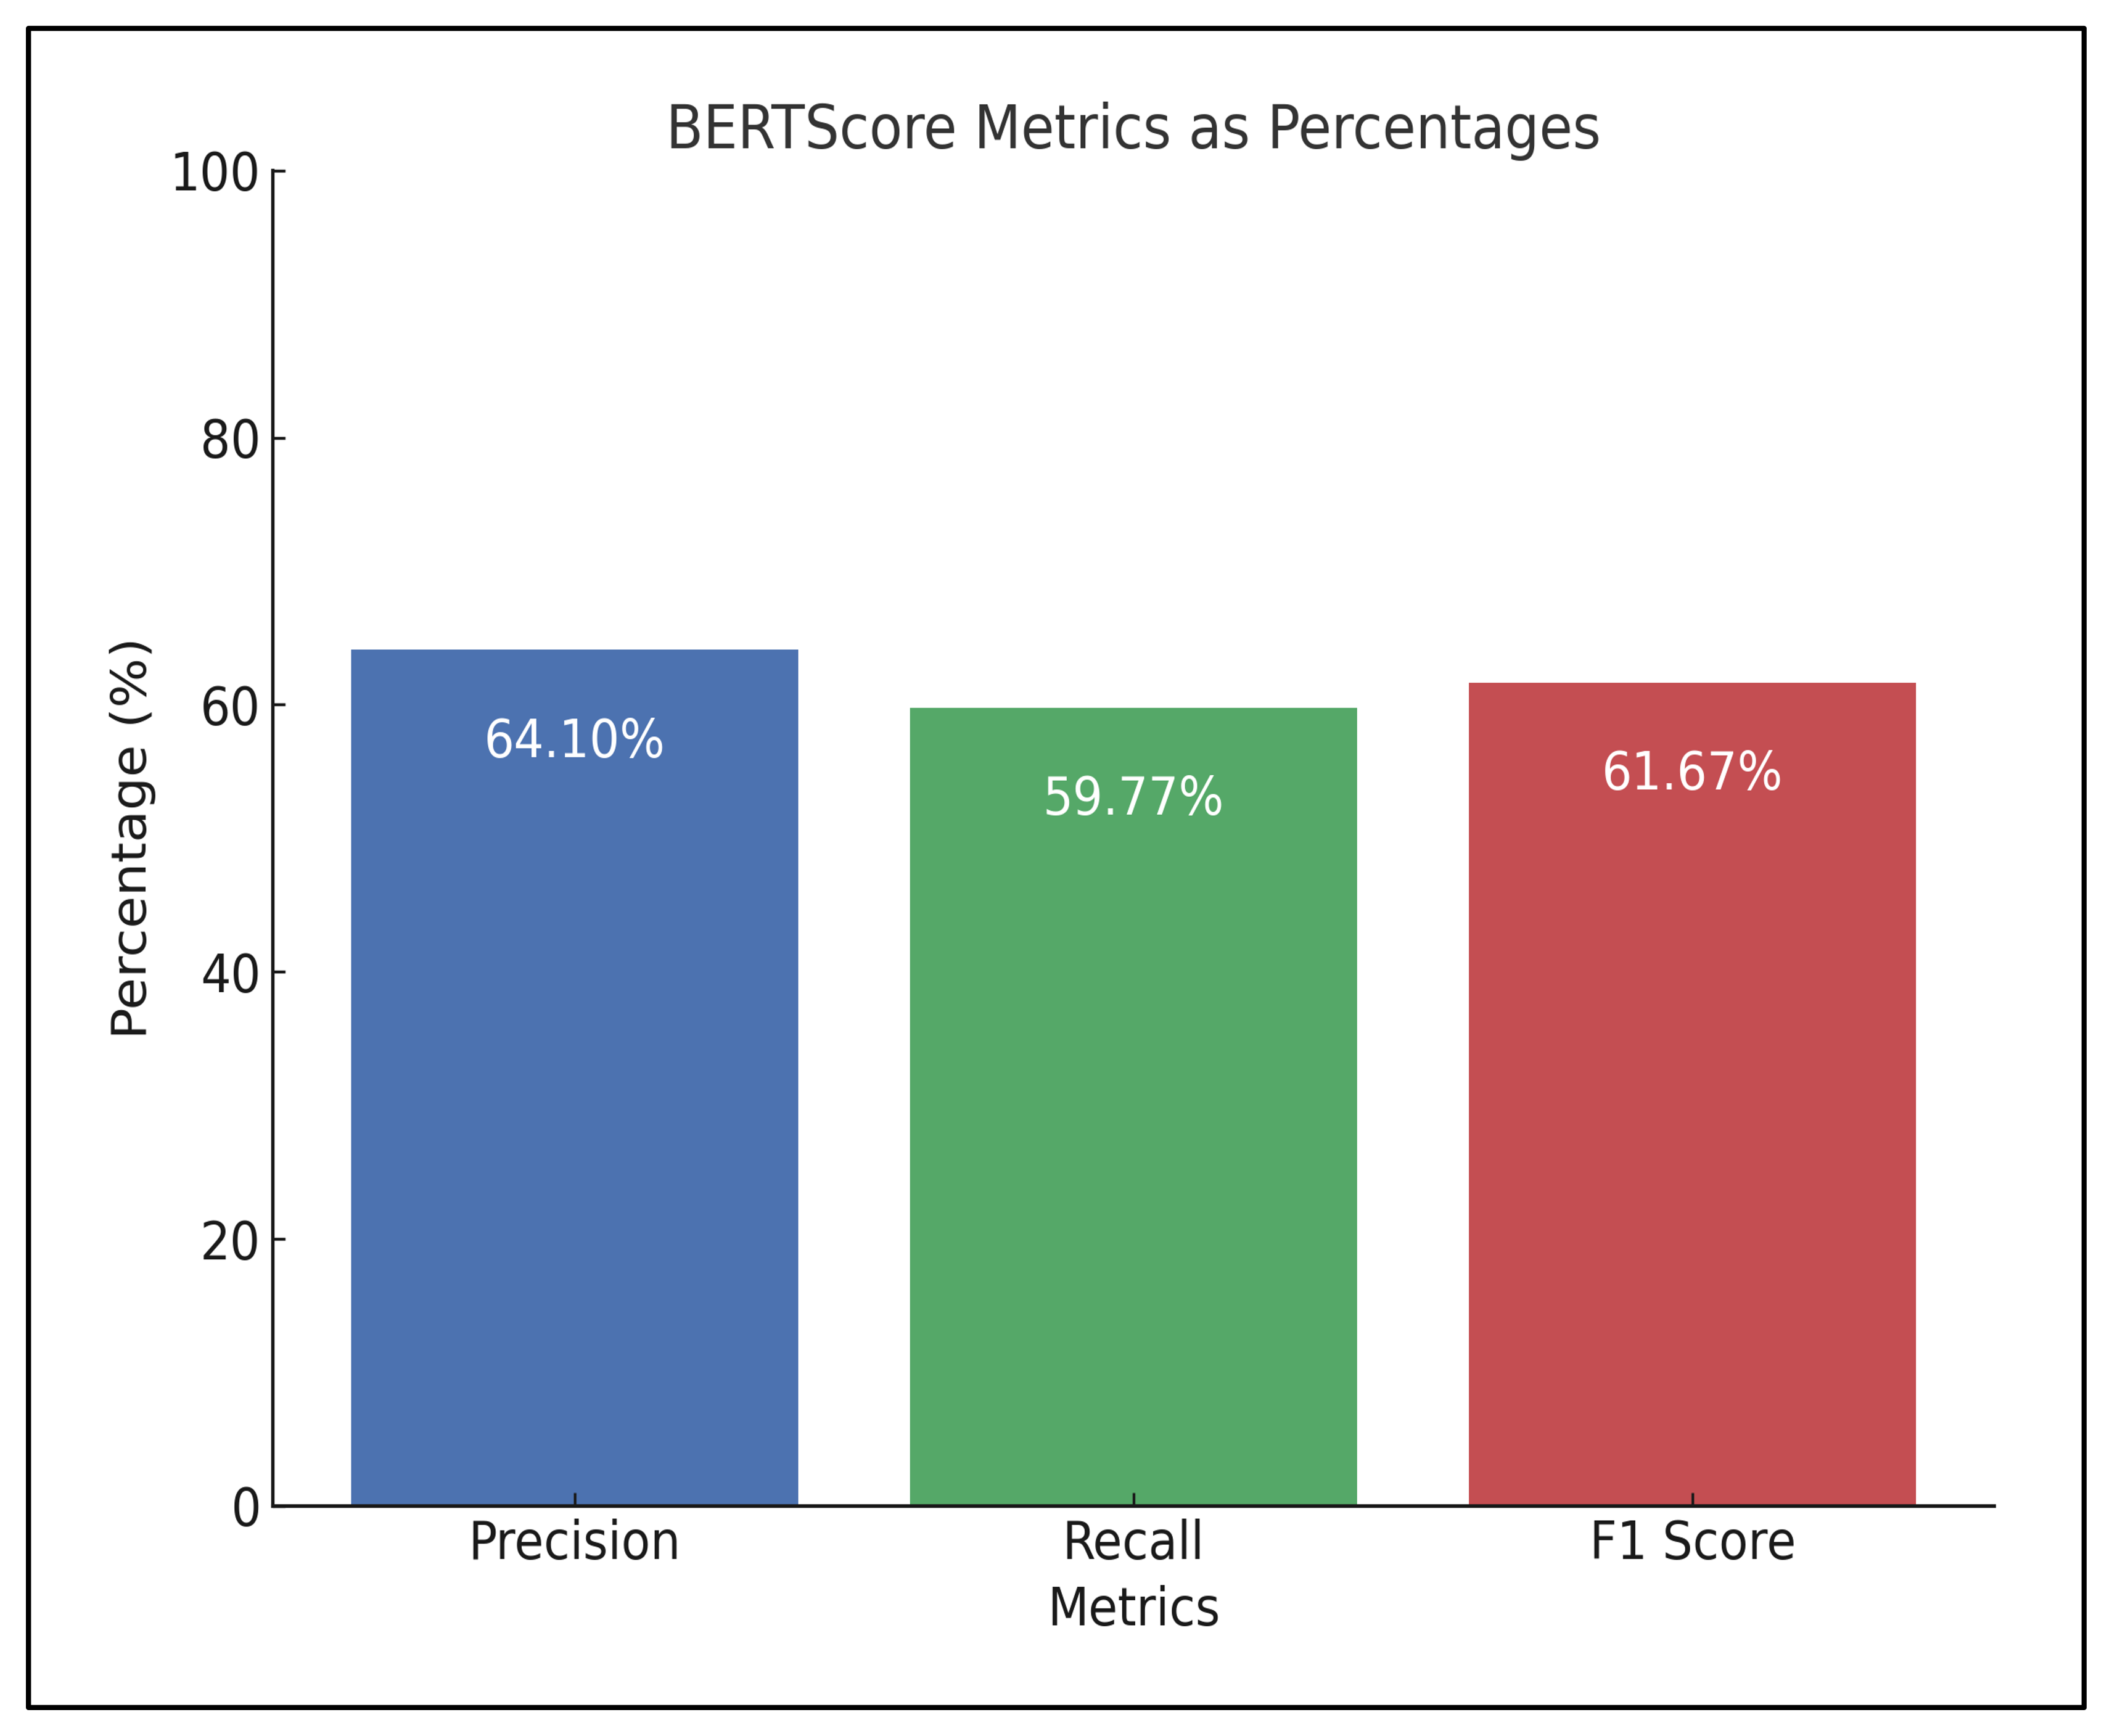
\includegraphics[width=3in]{bertscore.png}}
    \vspace{-0.4cm}
    \caption{BERTscore metrics result.}
    \label{bertscore}
\end{figure}
\indent Fig. \ref{bertscore} presents the metrics produced by 
BERTscore. The system achieved a 64.10\% precision, 59.77\%
recall, and 61.67\% F1 score. This means that the generated 
questions decently contains the original context from the 
reference. During runtime, 
it can be said that three out of the five generation 
would have decent adherance to the basis text. During 
analysis of the generated questions, there are 
questions that lack the relevant keywords from the 
reference question as well as the usual errors discussed in question 
validity. Moreover, there were students that utilized a 
different WH questions compared to the inference. Lastly, 
it was noticed that the questions generated by the system 
were considerably shorter, ranging in 9-14 words whereas 
the reference questions may have up to 17 words.
\section{Conclusion and Recommendations}
    \indent It was concluded that the system utilizing the T5 and TrOCR 
    pipeline was capable of performing AQG from handwritten lecture notes
    with satisfactory validity and relevance, but unpredictable in 
    lexical structure. \\
    \indent It is recommended that further research on 
    this implementation use better hardware. This will lead 
    to the usage of higher paramter count versions of T5 and TrOCR 
    which will improve the operation of the system. Lastly, it is 
    recommended that much attention is given to the preprocessing of 
    the image captures of handwritten notes to improve the word 
    capture accuracy through text enhancer LLMs or by utilizing 
    an alternative framework for OCR. 

\bibliographystyle{IEEEtran}
\bibliography{export}


\end{document}
